\documentclass[border=6pt]{standalone}
\usepackage{tikz}
\usepackage[edges]{forest}
\usetikzlibrary{arrows.meta,positioning,calc,decorations.pathreplacing,shapes.geometric}
\begin{document}
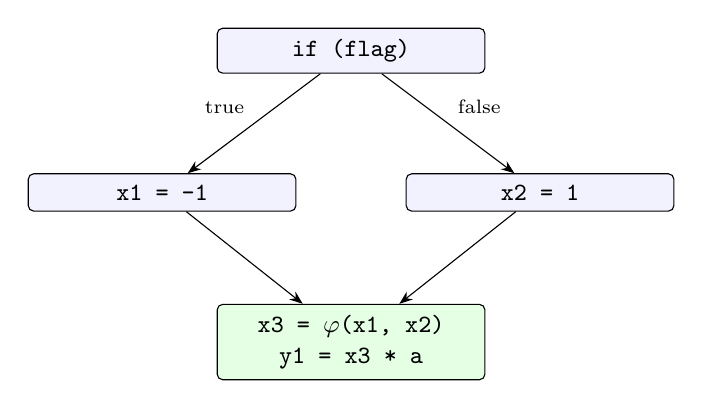
\begin{tikzpicture}[>=Stealth,font=\small,
 blk/.style={draw,rounded corners=2pt,fill=blue!5,align=center,minimum width=3.4cm,inner sep=4pt}]
\node[blk] (b1) at (0,0) {\texttt{if (flag)}};
\node[blk] (b2) at (-2.4,-1.8) {\texttt{x1 = -1}};
\node[blk] (b3) at (2.4,-1.8) {\texttt{x2 = 1}};
\node[blk,fill=green!10] (b4) at (0,-3.7) {\texttt{x3 = $\varphi$(x1, x2)}\\\texttt{y1 = x3 * a}};
\draw[->] (b1) -- node[above left,font=\scriptsize]{true} (b2);
\draw[->] (b1) -- node[above right,font=\scriptsize]{false} (b3);
\draw[->] (b2) -- (b4); \draw[->] (b3) -- (b4);
\end{tikzpicture}
\end{document}
